\documentclass[12pt]{article}
\usepackage[english]{babel}
\usepackage{natbib}
\usepackage{url}
\usepackage[utf8x]{inputenc}
\usepackage{amsmath}
\usepackage{graphicx}
\graphicspath{{images/}}
\usepackage{parskip}
\usepackage{fancyhdr}
\usepackage{subcaption}
\usepackage{relsize}
\usepackage{vmargin}
\setmarginsrb{3 cm}{2.5 cm}{3 cm}{2.5 cm}{1 cm}{1.5 cm}{1 cm}{1.5 cm}

\title{Statistical Pattern Recognition}								% Title
\author{94131091}								% Author
\date{\today}											% Date

\makeatletter
\let\thetitle\@title
\let\theauthor\@author
\let\thedate\@date
\makeatother

\pagestyle{fancy}
\fancyhf{}
\rhead{\theauthor}
\lhead{\thetitle}
\cfoot{\thepage}

\newcommand\numberthis{\addtocounter{equation}{1}\tag{\theequation}}
\newcommand{\gl}{^{>^{w_1}}_{<_{w_2}}}
\newcommand{\svector}[2]{\left[ \begin{matrix} #1 \\ #2 \end{matrix}\right]}
\newcommand{\smatrix}[4]{\left[ \begin{matrix} #1 & #2 \\ #3 & #4 \end{matrix}\right]}
\newcommand{\Pin}{\Pi_{i=1}^n}
\newcommand{\Sumn}{\Sigma_{i=1}^n}
\begin{document}

%%%%%%%%%%%%%%%%%%%%%%%%%%%%%%%%%%%%%%%%%%%%%%%%%%%%%%%%%%%%%%%%%%%%%%%%%%%%%%%%%%%%%%%%%

\begin{titlepage}
	\centering
    \vspace*{0.5 cm}
    
\includegraphics[scale = 0.4]{Imgs/logo.png}\\[1.0 cm]	% University Logo
    \textsc{\Large Computer Engineering \&\& IT Department\newline\newline Amirkabir University of Technology}\\[2.0 cm]	% University Name
%	\textsc{\large SPR\#1}\\[0.5 cm]				% Course Code
	\rule{\linewidth}{0.2 mm} \\[0.4 cm]
	{ \huge \bfseries \thetitle}\\
	\rule{\linewidth}{0.2 mm} \\[1.5 cm]
	
	\begin{minipage}{0.4\textwidth}
		\begin{flushleft} \large
			\emph{Submitted To:}\\
			Mohammad Rahmati\\
            Assoc. Professor\\
            Computer Engineering Department\\
			\end{flushleft}
			\end{minipage}~
			\begin{minipage}{0.4\textwidth}
            
			\begin{flushright} \large
			\emph{Submitted By :} \\
			Ahmad Asadi\\
            94131091\\
            Group-G1\\
            Fall-95\\
		\end{flushright}
        
	\end{minipage}\\[2 cm]
	
	
    
    
    
    
	
\end{titlepage}

%%%%%%%%%%%%%%%%%%%%%%%%%%%%%%%%%%%%%%%%%%%%%%%%%%%%%%%%%%%%%%%%%%%%%%%%%%%%%%%%%%%%%%%%%

\tableofcontents
\pagebreak

%%%%%%%%%%%%%%%%%%%%%%%%%%%%%%%%%%%%%%%%%%%%%%%%%%%%%%%%%%%%%%%%%%%%%%%%%%%%%%%%%%%%%%%%%

\section{Problem 1}
Let $\{x_k\}, k = 1,2, ... , n$ denote independent training data from one of the following densities.
Obtain the Maximum Likelihood estimate of $\theta$ in each case.

\begin{itemize}
\item $f(x_k, \theta) = \frac{x_k}{\theta^2}e^{-\frac{x_k^2}{2\theta^2}}, x_k \geq 0, \theta > 0$ \\ \\
We will first form likelihood function and then find the optimum value of $\theta$ maximizing it.
\begin{align*}
&l(\theta) = P(D|\theta) = \Pi_{i=1}^n P(X_i|\theta) = \Pi_{i=1}^n \frac{x_i^2}{\theta^2} e^{-\frac{x_i^2}{2\theta^2}} = \frac{1}{\theta^{2n}}\Pi_{i=1}^n (x_i^2 e^{-\frac{x_i^2}{2\theta^2}})\\
&\rightarrow l(\theta) = \frac{1}{\theta^{2n}}(\Pi_{i=1}^n x_i^2 )e^{\Sigma_{i=1}^n -\frac{x_i^2}{2\theta^2}} \rightarrow ln (l(\theta)) = ln \frac{\Pi_{i=1}^n x_i^2}{\theta^{2n}} - \Sigma_{i=1}^n \frac{x_i^2}{2\theta^2}\\
& \nabla_\theta ln(l(\theta)) = \frac{-2n\theta^{-2n-1}\Pi_{i=1}^n X_i}{\theta^{-2n}\Pi_{i=1}^nX_i} - 4\theta^{-3} \Sigma_{i=1}^n x_i^2 = \frac{-2n}{\theta} - 4\theta^{-3}\Sigma_{i=1}^nX_i^2 = 0\\
&\rightarrow \theta^* = \sqrt{\frac{2}{n} \Sigma_{i=1}^n X_i^2}
\end{align*}

\begin{center}
\line(1,0){250}
\end{center}
%%%%%%%%%%%%%%%%%%%%%%%%%%%%%%%%%%%%%%%%%%%%
\item $f(x_k, \theta) = \sqrt{\theta} x_k^{\sqrt{\theta} - 1}, 0 \leq x_k \leq 1, \theta > 0$ 

\begin{align*}
&l(\theta) = P(D|\theta) = \Pin \sqrt{\theta} X_i^{\sqrt{\theta} - 1} = \theta^\frac{n}{2} \Pin X_i^{\sqrt{\theta} - 1} \\
&\rightarrow ln(l(\theta)) = \frac{n}{2} ln(\theta) + (\sqrt{\theta} - 1)ln(\Pin X_i)\\
&\rightarrow \nabla_\theta ln(l(\theta)) = \frac{n}{2\theta} + \frac{1}{2} \theta^{-\frac{1}{2}}ln(\Pin X_i) = 0 \rightarrow \theta^* = (\frac{-n}{\Sumn ln X_i})^2
\end{align*}

\end{itemize}


\begin{center}
\line(1,0){450}
\end{center}

%%%%%%%%%%%%%%%%%%%%%%%%%%%%%%%%%%%%%%%%%%%%%%%%%%%%%%%%%%%%%%%%%%%%%%%%%%%%%%%%%%%%%%%%%

\section{Problem 2}
Let $x$ have uniform density:
\begin{align}
f_x(x,\theta) \propto U(0,\theta) = \left\{ \begin{array}{c c}
\mathlarger{\frac{1}{\theta}} & 0 \leq x \leq 1 \\
0 & otw
\end{array} \right.
\end{align}

\begin{enumerate}
\item Suppose that $n$ samples $D = \{x_1 , x_2 , \cdots , x_n \}$ are drawn independently according to
$f_x(x|\theta)$. Show that the maximum likelihood estimate for $\theta$ is $max [D]$, i.e., the
value of the maximum element in $D$.\\

Since all samples are drawn independently, we have:
\begin{equation}
P(D|\theta) = \Pin P(X_i|\theta)
\label{eq:2-1}
\end{equation}
According to proposed uniform density function, if there exists $X_i \in D$ such that $X_i < \theta$ then $P(X_i|\theta) = 0$, therefore according to \eqref{eq:2-1}, $P(D|\theta) = 0$. So the likelihood of such values of $\theta$ will be equal to zero, hence we can conclude that:
\begin{equation}
\forall \theta, \exists X_i \in D; X_i < \theta \Leftrightarrow l(\theta) = 0.
\label{eq:2-2}
\end{equation}
According to \eqref{eq:2-2}, it is meaningful to assume $\theta \geq max[D]$ to get regions of nonzero likelihood. Having uniform density in mind and considering $\theta \geq max[D]$ as the result of \eqref{eq:2-2}:
\begin{equation}
P(D|\theta) = \Pin P(X_i|\theta) = \frac{1}{\theta^n} 
\label{eq:2-3}
\end{equation}
As it is obviously clear, \eqref{eq:2-3} does not have optimal value globally but taking \eqref{eq:2-2} constraint into consideration yields $\theta^* = max[D]$, since the gradient of likelihood function is negative and so the likelihood function is monotonically decreasing in the range of $[max[D], +\inf)$. \\
Figure \ref{fig:2-1} represents the proposed likelihood function in \eqref{eq:2-3}.
\begin{figure}[h]
\centering 
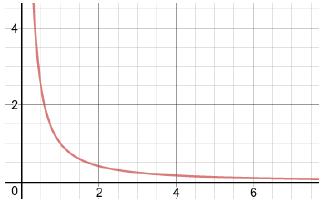
\includegraphics[scale=0.4]{Imgs/2-1.png}
\caption{The proposed likelihood function in \ref{eq:2-3}}
\label{fig:2-1}
\end{figure}


\begin{center}
\line(1,0){250}
\end{center}
%%%%%%%%%%%%%%%%%%%%%%%%%%%%%%%
\item Suppose that $n = 5$ point are drawn from the distribution and the maximum value
of which happens to be $max x_k = 0.6$. Plot the likelihood function $f_x(D|\theta)$ in the
range $0 \leq \theta \leq 1$. Explain in words why you do not need to know the values of
other four points.\\
As discussed in the first part, the likelihood function $f_x(D|\theta)$ is zero when $\theta < max[D]$, because the conditional probability of each sample is represented as $P(X_i|\theta) \propto U(0,\theta)$. \\
giving more details, whenever $\theta < max[D]$, there exists at least one sample $X_i \in D$ such that $\theta < X_i$. Therefore, taking the fact that all samples are drawn from a uniform distribution, $P(X_i | \theta ) = 0$ which implies that $P(D|\theta) = 0$. Keeping this fact in mind, knowing the values of points rather than the maximum one, is absolutely useless.\\
On the other cases in which $\theta \leq max[D]$, we have $P(D|\theta) = \frac{1}{\theta^n}$. As here $n = 5$, the likelihood function will be in the form of $P(D|\theta) = \frac{1}{\theta^5}$. \\
Figure \ref{fig:2-2} displays the likelihood function of this problem.
\begin{figure}[h]
\centering
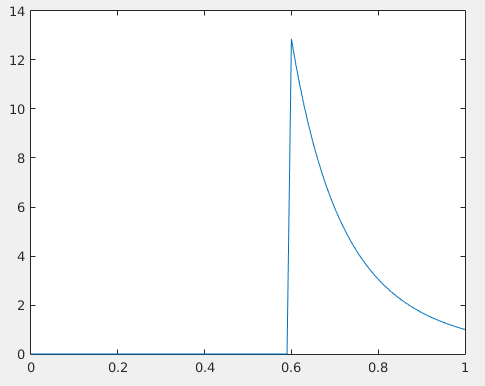
\includegraphics[scale=0.4]{Imgs/2-2.png}
\caption{The likelihood functon of the problem 2\_2.}
\label{fig:2-2}
\end{figure}

\end{enumerate}

\begin{center}
\line(1,0){450}
\end{center}

%%%%%%%%%%%%%%%%%%%%%%%%%%%%%%%%%%%%%%%%%%%%%%%%%%%%%%%%%%%%%%%%%%%%%%%%%%%%%%%%%%%%%%%%%
\section{Problem 3}
Consider the standard two class SVM with the hinge loss. Argue that under a given value
of regularization parameter:
\begin{center}
Leave-one-out-Error $< \frac{\#SVs}{l}$
\end{center}
Where $l$ is the size of training data and $\#SVs$ is the number of support vectors obtained by
training SVM on the entire set of training data.
\\
To calculate leave-one-out-error, we first train SVM on $n - 1$ training samples and test the other remaining one. If the remaining point is a support vector for the full $n$ sample case, then there will be an error. Note that if we can find a transformation $\phi(.)$ that well separates the data, then Leave-one-out-Error $< \frac{\#SVs}{l}$ shows that the expected error rate will be lower.\\
This bound is also independent of the dimensionality of the space of transformed vectors determined by $\phi(.)$.

\begin{center}
\line(1,0){450}
\end{center}

%%%%%%%%%%%%%%%%%%%%%%%%%%%%%%%%%%%%%%%%%%%%%%%%%%%%%%%%%%%%%%%%%%%%%%%%%%%%%%%%%%%%%%%%%
\section{Problem 4}
Consider the 2-dimensional points and their classification (‘+’ or ‘-‘) below:

\begin{table}[h]
\centering
\begin{tabular}{| c  c | c |}
\hline
x & y & class \\
\hline 
0 & 4 & + \\
8 & 3 & + \\
6 & -2 & - \\
4 & 0 & - \\
2 & 1 & -\\ \hline
\end{tabular}
\end{table}

\begin{itemize}
\item  The points with classification ‘+’ and ‘-’ corresponds to the point sets $M_+$ and $M_-$ ,
respectively. Draw the points and determine first whether or not the sets $M_+$ and $M_-$ are linearly separable. And then whether or not the two sets are linearly separable by a 2-
dimensional perceptron.\\
To determine that if a data set containing samples of two different classes is linearly separable, it is sufficient to check whether there exists a separating line such that $a^TX + w_0 ._{<_{M_-}}^{>^{M_+}} 0$.

Figure \ref{fig:4-1} displays the given data points and a proposed separating line $0.5x_1 + x_2 - 3 = 0 $. As it is illustrated in this figure, the given data set is linearly separable.

\begin{figure}[h]
\centering
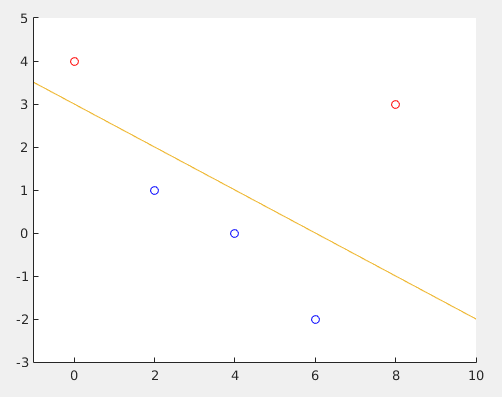
\includegraphics[scale=0.4]{Imgs/4-1.png}
\caption{Given dataset and separating line in problem 4. The red points are points from $M_+$ and the blue points are points from $M_-$.}
\label{fig:4-1}
\end{figure}

Since, none of the separating lines will not cross the origin point, it is necessary to have bias terms augmented in perceptron model. Therefore, a 2-dimensional perceptron, without augmented bias terms, which is just able to draw lines crossing zero point, is not able to classify given dataset.\\

Another way rather than drawing line graphically is to first negate all samples from one of the classes, for example instances from class $M_-$, and then find any vector $a$ such that $a^Ty > 0$ for all $y \in D$, denoting dataset by $D$.\\
Negating all samples from second class and considering 3-dimensional data samples, in bias augmented model, yields following vector:
\[
a = [-3 10 -4]^T
\]
Calculation of this vector is illustrated in table \ref{tbl:4-1} and figure \ref{fig:4-2} represents the underlying line by it.

\begin{figure}[h]
\centering
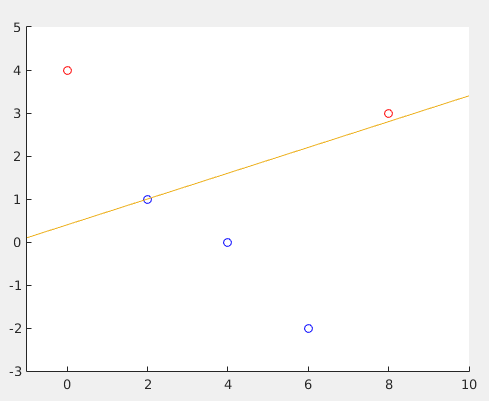
\includegraphics[scale=0.4]{Imgs/4-3.png}
\caption{Given dataset and separating line by a 3-dimensional perceptron in problem 4. The red points are points from $M_+$ and the blue points are points from $M_-$.}
\label{fig:4-1}
\end{figure}



\begin{center}
\line(1,0){250}
\end{center}
%%%%%%%%%%%%%%%%%%%%%
\item  Manually execute the perceptron learning algorithm on this dataset. Based on your answer
from part (a) decide whether or not you need a bias. Use a vector of all ones as the initial
weight vector. Write all the intermediate results of your perceptron computation in a table.\\

We first negate all the samples of class $M_-$ and then augment a bias component to perceptron weights and an augmented 1 to data instances. It is obviously clear that augmented 1s in samples from $M_-$ will be negated too.\\

Table \ref{tbl:4-1} illustrates all steps of perceptron learning algorithm. In all cases that $a^Ty < 0$ we will consider a misclassification and we will consider all $y \in D$ in which $a^T y = 0$, $y \in < M_-$. 

\begin{table}
\centering
\caption{Perceptron learning algorithm steps in case of considering bias components.}
\label{tbl:4-1}
\begin{tabular}{c | c | c | | c | c | c | | c }
$y_1$ & $y_2$ & $y_3$ & $a_1$ & $a_2$ & $a_3$ & $a^Ty$ \\
\hline \hline
0 &4 &1 &1 &1 &1 &$>$0\\ 
8 &3 &1 &1 &1 &1 &$>$0\\ 
-6 &2 &-1 &1 &1 &1 &$<$0\\
-4 &0 &-1 &-5 &3 &0 &$>$0\\
-2 &-1 &-1 &-5 &3 &0 &$>$0\\ \hline \hline
0 &4 &1 &-5 &3 &0 &$>$0\\
8 &3 &1 &-5 &3 &0 &$<$0\\
-6 &2 &-1 &3 &6 &1 &$<$0\\
-4 &0 &-1 &-3 &8 &0 &$>$0\\
-2 &-1 &-1 &-5 &7 &-1 &$<$0\\\hline \hline
0 &4 &1 &-5 &7 &-1 &$>$0\\
8 &3 &1 &-5 &7 &-1 &$<$0\\
-6 &2 &-1 &3 &10 &0 &$>$0\\
-4 &0 &-1 &3 &10 &0 &$<$0\\
-2 &-1 &-1 &-1 &10 &-1 &$<$0\\ \hline \hline
0 &4 &1 &-3 &9 &-2 &$>$0\\
8 &3 &1 &-3 &9 &-2 &$>$0\\
-6 &2 &-1 &-3 &9 &-2 &$>$0\\
-6 &2 &-1 &-3 &9 &-2 &$>$0\\
-4 &0 &-1 &-3 &9 &-2 &$>$0\\
-2 &-1 &-1 &-3 &9 &-2 &$<$0\\ \hline \hline
0 &4 &1 &-5 &8 &-3 &$>$0\\
8 &3 &1 &-5 &8 &-3 &$<$0\\
-6 &2 &-1 &3 &11 &-2 &$>$0\\
-4 &0 &-1 &3 &11 &-2 &$<$0\\
-2 &-1 &-1 &-1 &11 &-3 &$<$0\\ \hline \hline
0 &4 &1 &-3 &10 &-4 &$>$0\\
8 &3 &1 &-3 &10 &-4 &$>$0\\
-6 &2 &-1 &-3 &10 &-4 &$>$0\\
-4 &0 &-1 &-3 &10 &-4 &$>$0\\
-2 &-1 &-1 &-3 &10 &-4 &$=$0\\\hline
\end{tabular}
\end{table}


\begin{center}
\line(1,0){250}
\end{center}
%%%%%%%%%%%%%%%%%%%%%
\item  Give the linear function that has been learned by this perceptron.\\
Linear function representing by this perceptron is presented in equation \eqref{eq:4-1}
\begin{equation}
f(X) = -3X_1 + 10 X_2 -4 .^{>^{M_+}}_{\leq_{M_-}} 0
\label{eq:4-1}
\end{equation}

\begin{center}
\line(1,0){250}
\end{center}
%%%%%%%%%%%%%%%%%%%%%
\item  Classify point (5,2) base on the trained perceptron.\\
Computing the value of $f([5,2])$:
\begin{align*}
f([5,2]) = -15 + 20 -4 = 1 > 0
\end{align*}
So the point (5,2) is in $M_+$.
\end{itemize}
%%%%%%%%%%%%%%%%%%%%%%%%%%%%%%%%%%%%%%%%%%%%%%%%%%%%%%%%%%%%%%%%%%%%%%%%%%%%%%%%%%%%%%%%%


\begin{center}
\line(1,0){450}
\end{center}

%%%%%%%%%%%%%%%%%%%%%%%%%%%%%%%%%%%%%%%%%%%%%%%%%%%%%%%%%%%%%%%%%%%%%%%%%%%%%%%%%%%%%%%%%
\section{Computer Exercises}
All the scripts are properly named and attached to the submitted file.
\subsection{Exercise 1}
\begin{enumerate}
\item The criterion function used in gradient descent method is the $l2-norm$ of the transformation matrix $a$ and for preceptron is the number of misclassified samples. Figure \ref{fig:ce1-1} displays criterion function changes over iterations for both algorithms.

\begin{figure}[h]
\centering 
\begin{subfigure}{0.4\textwidth}
	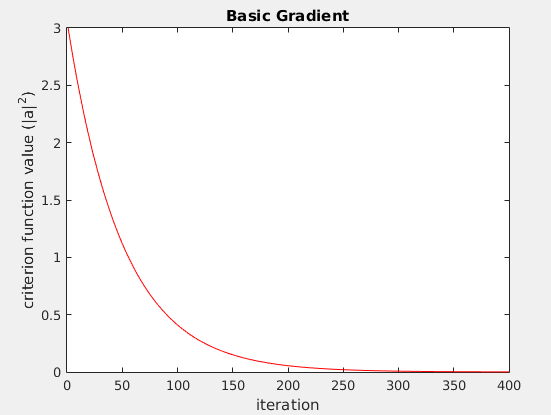
\includegraphics[scale=0.3]{Imgs/ce1-1.png}
	\caption{Basic gradient algorithm}
\end{subfigure}
\begin{subfigure}{0.4\textwidth}
	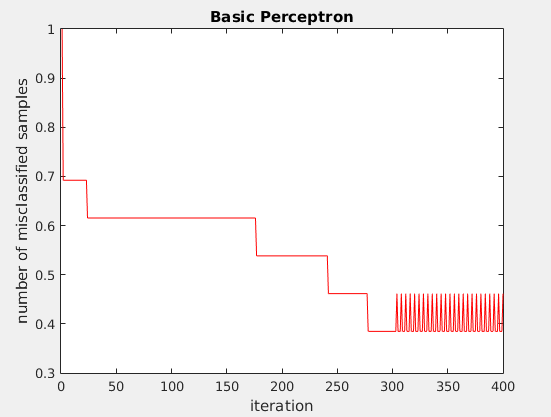
\includegraphics[scale=0.3]{Imgs/ce1-2.png}
	\caption{Basic perceptron algorithm}
\end{subfigure}
\caption{Criterion function changes over iterations in both perceptron and gradient algorithms.}
\label{fig:ce1-1}
\end{figure}

\item In basic gradient algorithm in each iteration there exists just 2 mathematical operations. Therefore after 400 iterations the estimated total number of mathematical operations would be 800. On the other hands, in basic perceptron algorithm there exists $1 + |Y|$ mathematical operations in each iteration, note that $|Y|$ is 1 if the current sample is misclassified and 0 otherwise. So the estimated total mathematical operations should be $\#iterations + \#misclassifiedSamples$. The estimated number is $300 + 2700 = 3000$.
\end{enumerate}

\begin{center}
\line(1,0){250}
\end{center}

%%%%%%%%%%%%%%%%%%%%%%%%%%%%%%%%%%%%%%%%%%%%%%%%%%%%%%%%%%%%%%%%%%%%%%%%%%%%%%%%%%%%%%%%%
\subsection{Exercise 2}

As it is clearly obvious from distribution of samples from 3 classes, in cases that separabality is higher, the perceptron algorithm can reach the optimum value faster and the convergence speed would be higher. Figure \ref{fig:ce2-1} illustrates classification error during epochs of perceptron in two cases. The right side figure is error in classifying $W_1$ and $W_2$ and the left side figure illustrates that of $W_2$ and $W_3$.

\begin{figure}[h]
\centering
\begin{subfigure}{0.4\textwidth}
	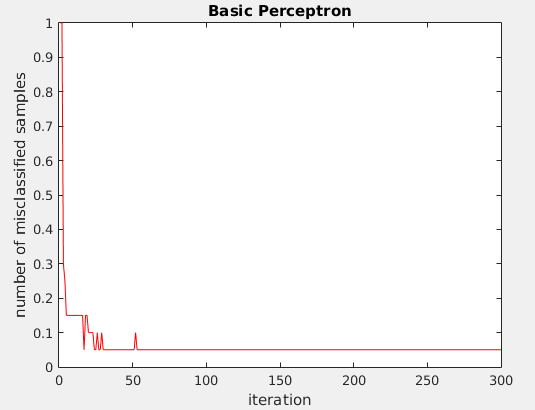
\includegraphics[scale=0.3]{Imgs/ce2-1.png}
	\caption{classification of $W_1$ and $W_2$}
\end{subfigure}
\begin{subfigure}{0.4\textwidth}
	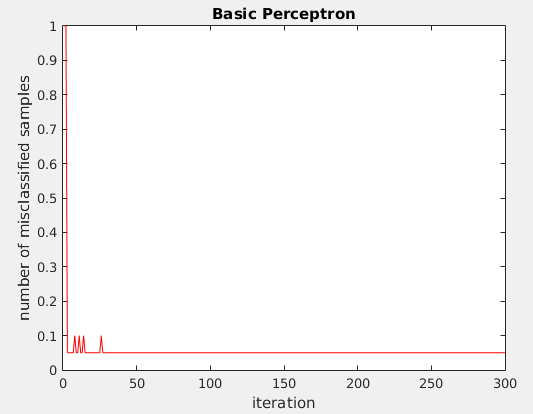
\includegraphics[scale=0.3]{Imgs/ce2-3.png}
	\caption{classification of $W_2$ and $W_3$}
\end{subfigure}
\caption{Classification error in cases of different levels of separabalities in data.}
\label{fig:ce2-1}

\end{figure}

\begin{center}
\line(1,0){250}
\end{center}

%%%%%%%%%%%%%%%%%%%%%%%%%%%%%%%%%%%%%%%%%%%%%%%%%%%%%%%%%%%%%%%%%%%%%%%%%%%%%%%%%%%%%%%%%
\subsection{Exercise 9}
The script is implemented in MATLAB and its source file is attached to submitted zip file.
\end{document}